\chapter[Идентификация линейных стохастических систем второго типа]{%
  Идентификация линейных стохастических систем второго типа
}

\section{Математическая модель идентифицируемой системы}

Для обеспечения наглядности сравнения рассматривался случай идентификации скалярной системы.
В этом случае функция регрессии принимает простой вид:
\begin{equation}
  \psi = \alpha + \beta \xi,
  \label{eq:fun_linear_scalar}
\end{equation}
где \( \alpha, \beta \) "--- постоянная составляющая и коэффициент усиления "---
параметры системы. Модель задачи идентификации выглядит следующим образом:
\begin{equation}
  \label{eq:model_linear_scalar}
  \begin{aligned}
  h &= \alpha + \beta \xi, \\
  x &= \xi + \varepsilon_x, \\
  y &= h + \varepsilon_y,
  \end{aligned}
\end{equation}
где \( \xi, h \) "--- фактические значения входной и выходной переменной, \par
\( \alpha, \beta \) "--- фактические значения параметров объекта, \par
\( x, y \) "--- измеренные значения входной и выходной переменной, \par
\( \varepsilon_x, \varepsilon_y \) "--- независимые ошибки измерений значений входной и
выходной переменной, распределенные по нормальному закону:
\(
\varepsilon_x = N(0, \sigma_{\varepsilon_x}),
\varepsilon_y = N(0, \sigma_{\varepsilon_y})
\).

Данная модель использовалась для генерации наблюдений входа и выхода системы,
на основании которых были получены оценки её параметров методами на основе
классического и симметричного критериев аппроксимации.
Значения \( \xi_i \) выбирались из равномерного в \( [0, 10] \) распределения.
Для получения каждой оценки \( \hat{\alpha}, \hat{\beta} \) использовались результаты
ста наблюдений \( ( x_i, y_i ), i = \overline{1, n}, n = 100 \).

\section{Алгоритмы методов идентификации}

\subsection{Метод наименьших квадратов}

Метод наименьших квадратов ставит своей целью минимизировать сумму вертикальных расстояний
от аппроксимирующей функции (в линейном случае "--- гиперплоскости) до результатов наблюдений.
Это соответствует использованию классического критерия идентификации:
\begin{equation*}
  \rho_{\text{к}} = \sum_i \rho_{\text{к}_i} \rightarrow \min.
\end{equation*}

Пусть \( y \) "--- вектор-столбец наблюдений выходной переменной \( \eta \),
а \( X \) "--- \( (r \times n) \)-матрица измерений вектора \( \xi \)
(\( r \) строк матрицы представляют собой векторы значений входных переменных в данном наблюдении,
а \( n \) столбцов "--- векторы значений данной входной переменной во всех наблюдениях).

Алгоритм получения МНК-оценок параметров линейной скалярно-векторной функции регрессии сводится
к вычислению значения вектора~\cite{wiki_lse}
\begin{equation*}
  \hat{\theta} = (X^{T}X)^{-1}X^{T} y.
\end{equation*}

Выполнение этого алгоритма требует времени, линейно зависящего от числа измерений \( O(n) \),
при выполнении реалистичного условия \( n \gg r \).

\vspace{2\baselineskip}
\subsection{Метод симметричной аппроксимации}

Метод симметричной аппроксимации минимизирует сумму перпендикулярных расстояний
от аппроксимирующей гиперплоскости до результатов наблюдений.
Это соответствует использованию симметричного критерия идентификации:
\begin{equation*}
  \rho_{\text{с}} = \sum_i \rho_{\text{с}_i} \rightarrow \min.
\end{equation*}

Пусть \( X \) "--- \( (m \times n) \)-матрица измерений.
Первые \( r \) и последние \( m - r \) строк этой матрицы представляют собой векторы наблюдений
входных и выходных переменных соответственно,
а столбцы соответствуют векторам \( X_i \) значений переменных в данном наблюдении.

Алгоритм расчета оценок параметров линейной функции регрессии
методом симметричной аппроксимации выглядит следующим образом~\cite{mukha_2016}:
\begin{enumerate}
\item Рассчитываются выборочные моменты случайного вектора наблюдений входных и выходных переменных:
  \begin{equation*}
    \hat{A} = \dfrac{1}{n} \sum_{i=1}^n X_i, \quad
    \hat{D} = \dfrac{1}{n}  \sum_{i=1}^n (X_i - A) (X_i - A)^T.
  \end{equation*}
\item Формируется матрица \( P \), состоящая из собственных векторов матрицы \( \hat{D} \),
  расположенных в порядке убывания соответствующих им собственных чисел.
\item Формируются матрица \( C \), состоящая из \( r \) первых столбцов матрицы
  \( P \). Выполняется разбиение матриц \( X \), \( \hat{A} \) и \( C \) на блоки:
  \begin{equation*}
    C =
    \begin{pmatrix}
      C_r \\
      C_{m-r}
    \end{pmatrix}, \quad
    X =
    \begin{pmatrix}
      X_r \\
      X_{m-r}
    \end{pmatrix}, \quad
    \hat{A} =
    \begin{pmatrix}
      \hat{A}_r \\
      \hat{A}_{m-r}
    \end{pmatrix}.
  \end{equation*}
  Таким образом, матрицы \( C_r \) и \( X_r \) содержат первые \( r \) строк матриц
  \( C \) и \( X \) соответственно,
  а \( C_{m-r} \) и \( X_{m-r} \) "--- последние \( m - r \) строк этих матриц.
  Вектор \( \hat{A}_r \) содержит первые \( r \),
  а \( \hat{A}_{m-r} \) "--- последние \( m - r \) элементов вектора \( \hat{A} \).
\item Рассчитываются значения оценок параметров зависимости~\eqref{eq:fun_linear_scalar}:
  \begin{equation*}
    \begin{aligned}
      \hat{\beta} &= C_{m-r} (C_r)^{-1}, \\
      \hat{\alpha} &= \hat{A}_{m-r} - \hat{\beta} \hat{A}_r.
    \end{aligned}
  \end{equation*}
\end{enumerate}

Подобно МНК, асимптотическая сложность этого алгоритма также составляет \( O(n) \),
считая \( n \gg m \).


\section{Численный анализ точности методов идентификации}

\subsection{Точность оценивания параметров}

Было выполнено сравнение точности оценивания параметров
\( \hat{\alpha}, \hat{\beta} \) системы~\eqref{eq:model_linear_scalar},
полученных классической линейной регрессией и методом симметричной аппроксимации,
в зависимости от c.~к.~о. ошибок наблюдений \( \sigma_{\varepsilon_x}, \sigma_{\varepsilon_y} \).

В качестве величины, характеризующей точность оценивания параметров,
использовалось среднее Евклидово расстояние:
\begin{equation}
  \begin{aligned}
    d = \frac{1}{k} \sum_{j=1}^k \sqrt{(\hat{\alpha}_j - \alpha)^2 + (\hat{\beta}_j - \beta)^2}.
    \end{aligned}
  \label{eq:dst_linear_param}
\end{equation}

Расчеты расстояний~\eqref{eq:dst_linear_param} производились в узлах сетки значений
\( \sigma_{\varepsilon_x}, \sigma_{\varepsilon_y} \) в прямоугольнике
\( [0, 2] \times [0, 2] \) с шагом 0{,}1.
В каждом узле сетки вычислялось \( k = 100 \) оценок.

На рисунке~\ref{fig:comparison_linear_params}
показана зависимость разности величин~\eqref{eq:dst_linear_param},
полученных классической линейной регрессией и методом симметричной аппроксимации,
от с.к.о. ошибок наблюдений \( \sigma_{\varepsilon_x}, \sigma_{\varepsilon_y} \) при
различных значениях коэффициента усиления модели.
Графики данной зависимости при прочих значениях коэффициента усиления \( \beta \)
приведены в приложении~А.

Анализ данной зависимости показал, что
точность оценок параметров зависит от коэффициента усиления системы и
значений с.к.о. ошибок измерений входных и выходных переменных.
С ростом величины коэффициента усиления и с.к.о. ошибок измерения
метод симметричной аппроксимации дает более точные оценки,
чем классическая линейная регрессия.
При больших значениях коэффициента усиления \( \beta > 5 \)
точность симметричного оценивания значительно превосходит
точность классический подход (рисунок~\ref{fig:comparison_linear_params_beta-5}).

Для того, чтобы решить, какой метод даёт более точные оценки параметров,
предлагается использовать следующее эмпирическое правило: если
\begin{equation*}
  \sigma_{\varepsilon_y} < (0{,}7 + |\beta|) \sigma_{\varepsilon_x},
\end{equation*}
то метод симметричной аппроксимации оценивает параметры линейных стохастической систем
второго типа более точно, чем классическая линейная регрессия.

\begin{figure}[p]
  \begin{subfigure}[b]{\linewidth}
    \centering
    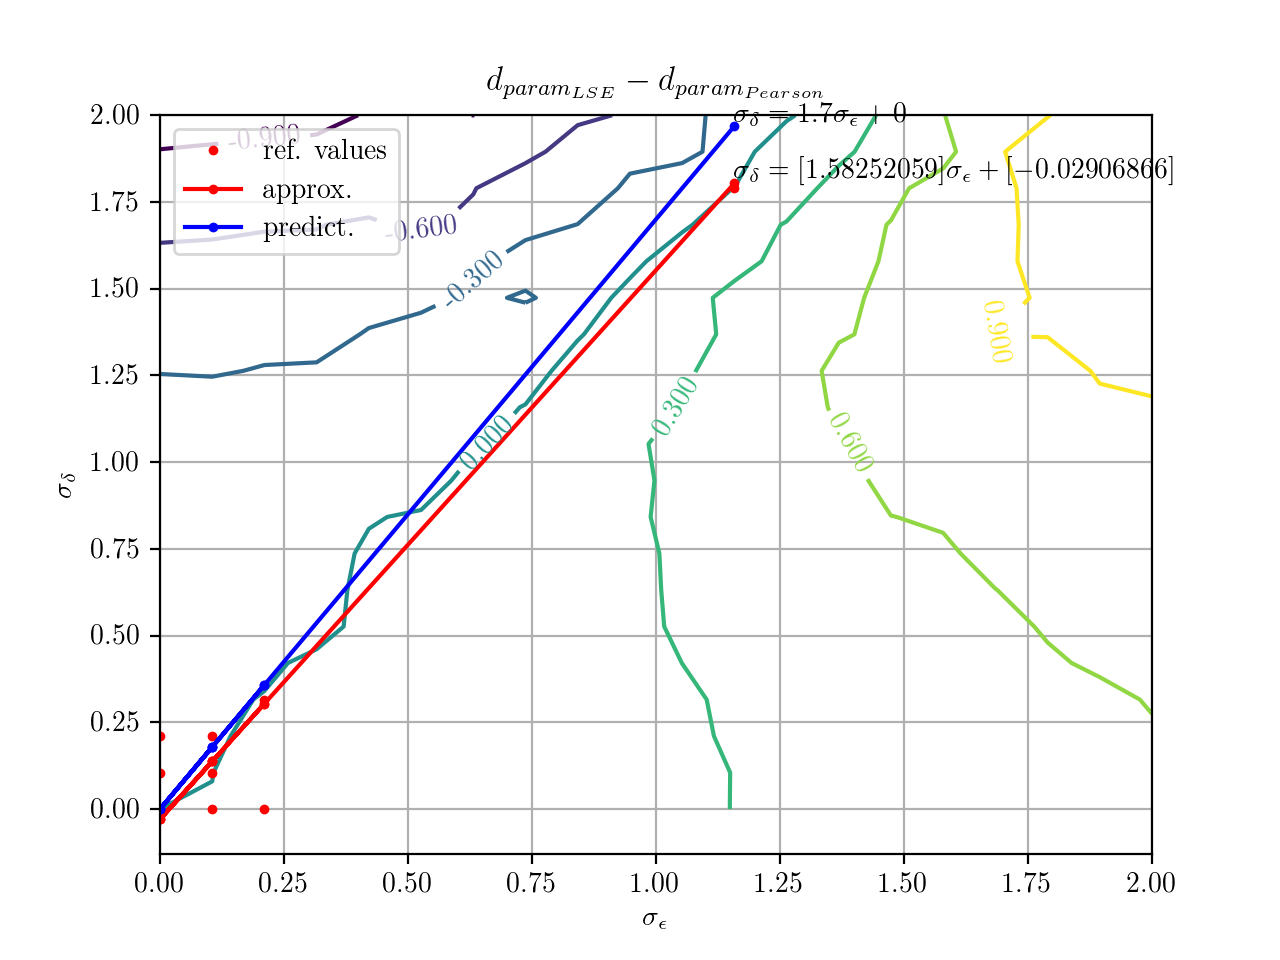
\includegraphics[width=150mm]{fig/linear/param/beta-1_param-accs-diff-approx.png}
    \caption{\( \beta = 1 \)}
  \end{subfigure}

  \begin{subfigure}[b]{\linewidth}
    \centering
    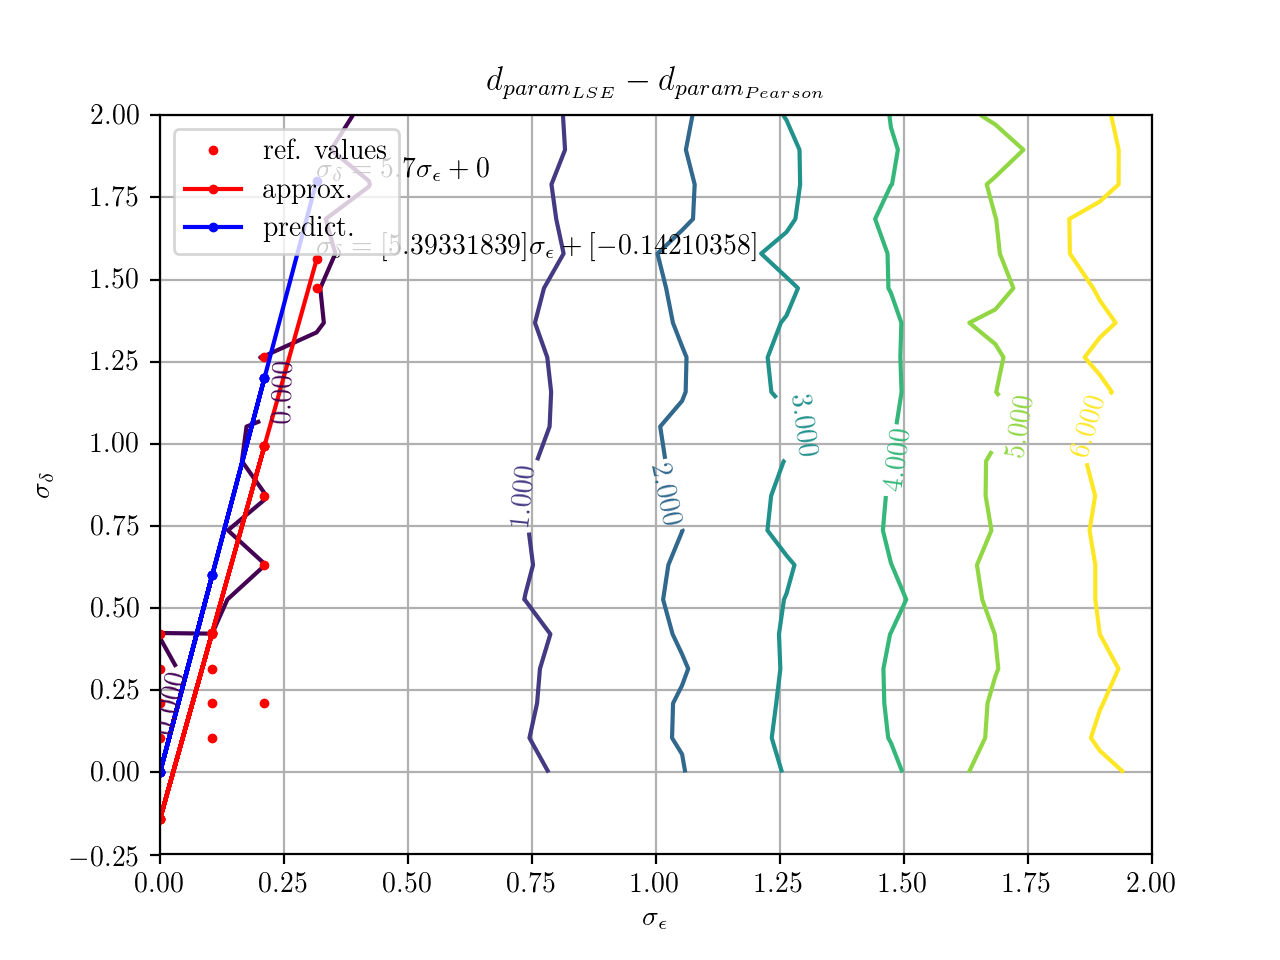
\includegraphics[width=150mm]{fig/linear/param/beta-5_param-accs-diff-approx.png}
    \caption{\( \beta = 5\)}\label{fig:comparison_linear_params_beta-5}
  \end{subfigure}
  \caption{Точность оценивания параметров модели}\label{fig:comparison_linear_params}
\end{figure}

\subsection{Точность прогнозирования наблюдений выхода}

Было выполнено сравнение точности прогнозирования наблюдений выхода по наблюдениям входа
системы~\eqref{eq:model_linear_scalar} со оценками параметров,
полученными классической линейной регрессией и методом симметричной аппроксимации,
в зависимости от c.~к.~о. ошибок наблюдений \( \sigma_{\varepsilon_x}, \sigma_{\varepsilon_y} \).

В качестве величины, характеризующей точность оценивания параметров,
использовалось среднее Евклидово расстояние:
\begin{equation}
  \begin{aligned}
    d = \frac{1}{k} \sum_{j=1}^k \sqrt{ \sum_{i=1}^n (\hat{\alpha}_j + \hat{\beta}_j x_{ij} - y_{ij})^2}.
    \end{aligned}
  \label{eq:dst_linear_predict}
\end{equation}

Расчеты расстояний~\eqref{eq:dst_linear_predict} производились в узлах сетки значений
\( \sigma_{\varepsilon_x}, \sigma_{\varepsilon_y} \) в прямоугольнике
\( [0, 2] \times [0, 2] \) с шагом 0{,}1.
В каждом узле сетки вычислялось \( k = 100 \) оценок.
Для получения каждой оценки \( \hat{\alpha}, \hat{\beta} \) использовались результаты
ста наблюдений \( ( x_i, y_i ), i = \overline{1, n}, n = 100 \).

Анализ зависимости разности величин~\eqref{eq:dst_linear_predict},
полученных классической линейной регрессией и методом симметричной аппроксимации,
от с.к.о. ошибок наблюдений \( \sigma_{\varepsilon_x}, \sigma_{\varepsilon_y} \) показал, что
классическая линейная регрессия дает более точные оценки фактических и наблюдаемых выходных
значений, чем метод симметричной аппроксимации,
во всем рассмотренном диапазоне значений коэффициента усиления системы и с.к.о. ошибок измерений.

Графики данной зависимости при различных значениях коэффициента усиления \( \beta \)
приведены в приложении~Б.

% точность оценок предсказания  зависит от коэффициента усиления системы и
% значений с.к.о. ошибок измерений входных и выходных переменных.
% С ростом величины коэффициента усиления и с.к.о. ошибок измерения
% метод симметричной аппроксимации дает более точные оценки,
% чем классическая линейная регрессия.
% При больших значениях коэффициента усиления \( \beta > 5 \)
% точность симметричного оценивания значительно превосходит
% точность классический подход (рисунок~\ref{fig:comparison_linear_params_beta-5}).

% На рисунке~\ref{fig:comparison_linear_predict}
% показана зависимость разности величин~\eqref{eq:dst_linear_predict},
% полученных классической линейной регрессией и методом симметричной аппроксимации,
% от с.к.о. ошибок наблюдений \( \sigma_{\varepsilon_x}, \sigma_{\varepsilon_y} \) при
% различных значениях коэффициента усиления модели.
% Графики данной зависимостей при прочих значениях коэффициента усиления \( \beta \)
% приведены в приложении~А.

% \begin{figure}[h]
%   \centering
%   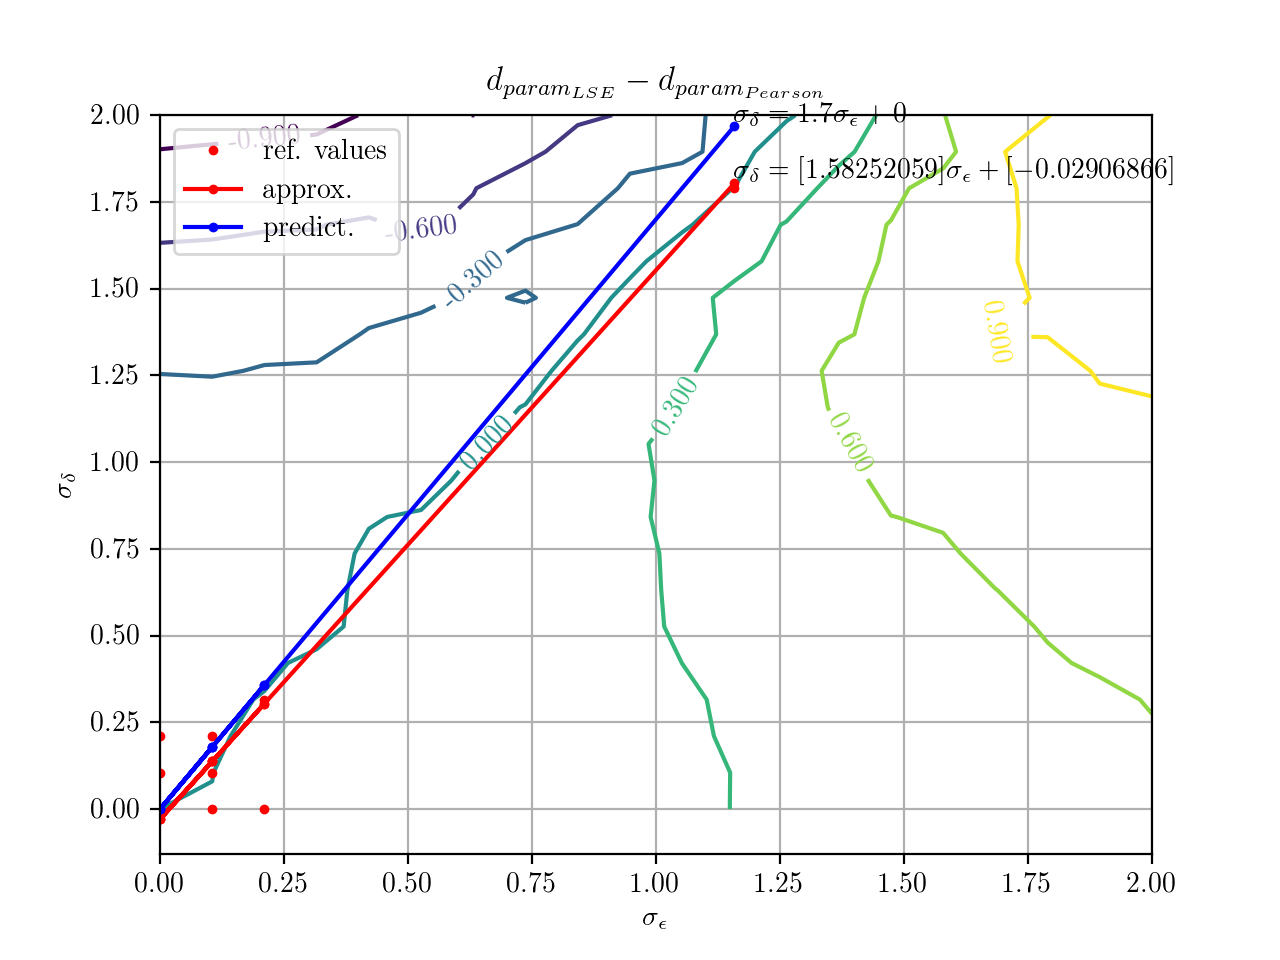
\includegraphics[width=150mm]{fig/linear/param/beta-1_param-accs-diff-approx.png}
%   \caption{\( \beta = 1 \)}
% \end{figure}

% \item Классическая линейная регрессия дает более точные оценки
%   фактических и наблюдаемых выходных значений, чем метод Пирсона,
%   во всем рассмотренном диапазоне значений коэффициента усиления системы и
%   с.к.о ошибок измерений.
% \end{enumerate}


% Требуется сравнить точность оценивания параметров
% \( \hat{\alpha}, \hat{\beta} \) и предсказания наблюдений выходных переменных \( y \)
% по наблюдениям входных переменных \( x \) от с.~к.~о. ошибок измерений
% \( \sigma_{\varepsilon_x}, \sigma_{\varepsilon_y} \),
% при использовании классического и симметричного критериев идентификации.

% Было выполнено сравнение точности оценок параметров
% \( \hat{\alpha}, \hat{\beta} \) системы~\eqref{eq:model_linear_scalar},
% полученных классической линейной регрессией и методом симметричной аппроксимации,
% в зависимости от c.~к.~о ошибок наблюдений \( \sigma_{\varepsilon_x}, \sigma_{\varepsilon_y} \).

% В качестве величин, характеризующих точность оценивания параметров,
% использовалось среднее Евклидово расстояние:
% \begin{equation}
%   \begin{aligned}
%     d = \frac{1}{k} \sum_{j=1}^k \sqrt{(\hat{\alpha}_j - \alpha)^2 + (\hat{\beta}_j - \beta)^2}.
%     \end{aligned}
%   \label{eq:dst_param}
% \end{equation}

% В качестве величин, характеризующих точность предсказания наблюдений выхода по наблюдениям входа,
% использовалось среднее Евклидово расстояние:
% \begin{equation}
%   \begin{aligned}
%     d = \frac{1}{k} \sum_{j=1}^k \sqrt{(\hat{\alpha}_j - \alpha)^2 + (\hat{\beta}_j - \beta)^2}.
%     \end{aligned}
%   \label{eq:dst_param}
% \end{equation}

% Расчеты расстояний~\eqref{eq:dst_param} производились в узлах сетки значений
% \( \sigma_{\varepsilon_x}, \sigma_{\varepsilon_y} \) в прямоугольнике
% \( [0, 2] \times [0, 2] \) с шагом 0{,}1.
% В каждом узле сетки вычислялось \( k = 100 \) оценок.


% Постановка задачи.
% Точность сравнения параметров и точность предсказания.
% Условия моделирования.
% Графики.
% Результаты (таблица)?
% Выводы.

% Матричное представление такой модели имеет вид:
% \begin{equation*}
%   y = X \theta + \varepsilon.
% \end{equation*}

% Вектор оценок выходной переменной и вектор остатков регрессии равны
% \( \hat{y} = X \theta, \) и \( e = y - \hat{y} = y - X \theta \) соответственно.
% Сумма квадратов остатков регрессии равна \( RSS = e^T e = (y - X \theta)^T (y - X \theta) \).
% Дифференцируя эту функцию по вектору параметров \( \theta \) и приравняв производные к нулю,
% получим систему уравнений:
% \begin{equation*}
%   (X^T X)b = X^T y.
% \end{equation*}

% Решение этой системы уравнений дает общую формулу МНК-оценок:
% \begin{equation}
%   \hat{\theta} = (X^{T}X)^{-1}X^{T} y.
% \end{equation}

% {\color{red}
%   Пару слов о свойствах и применимости МНК?
%   Ограничения?
% }
